\begin{figure}[thb]
    \begin{center}
      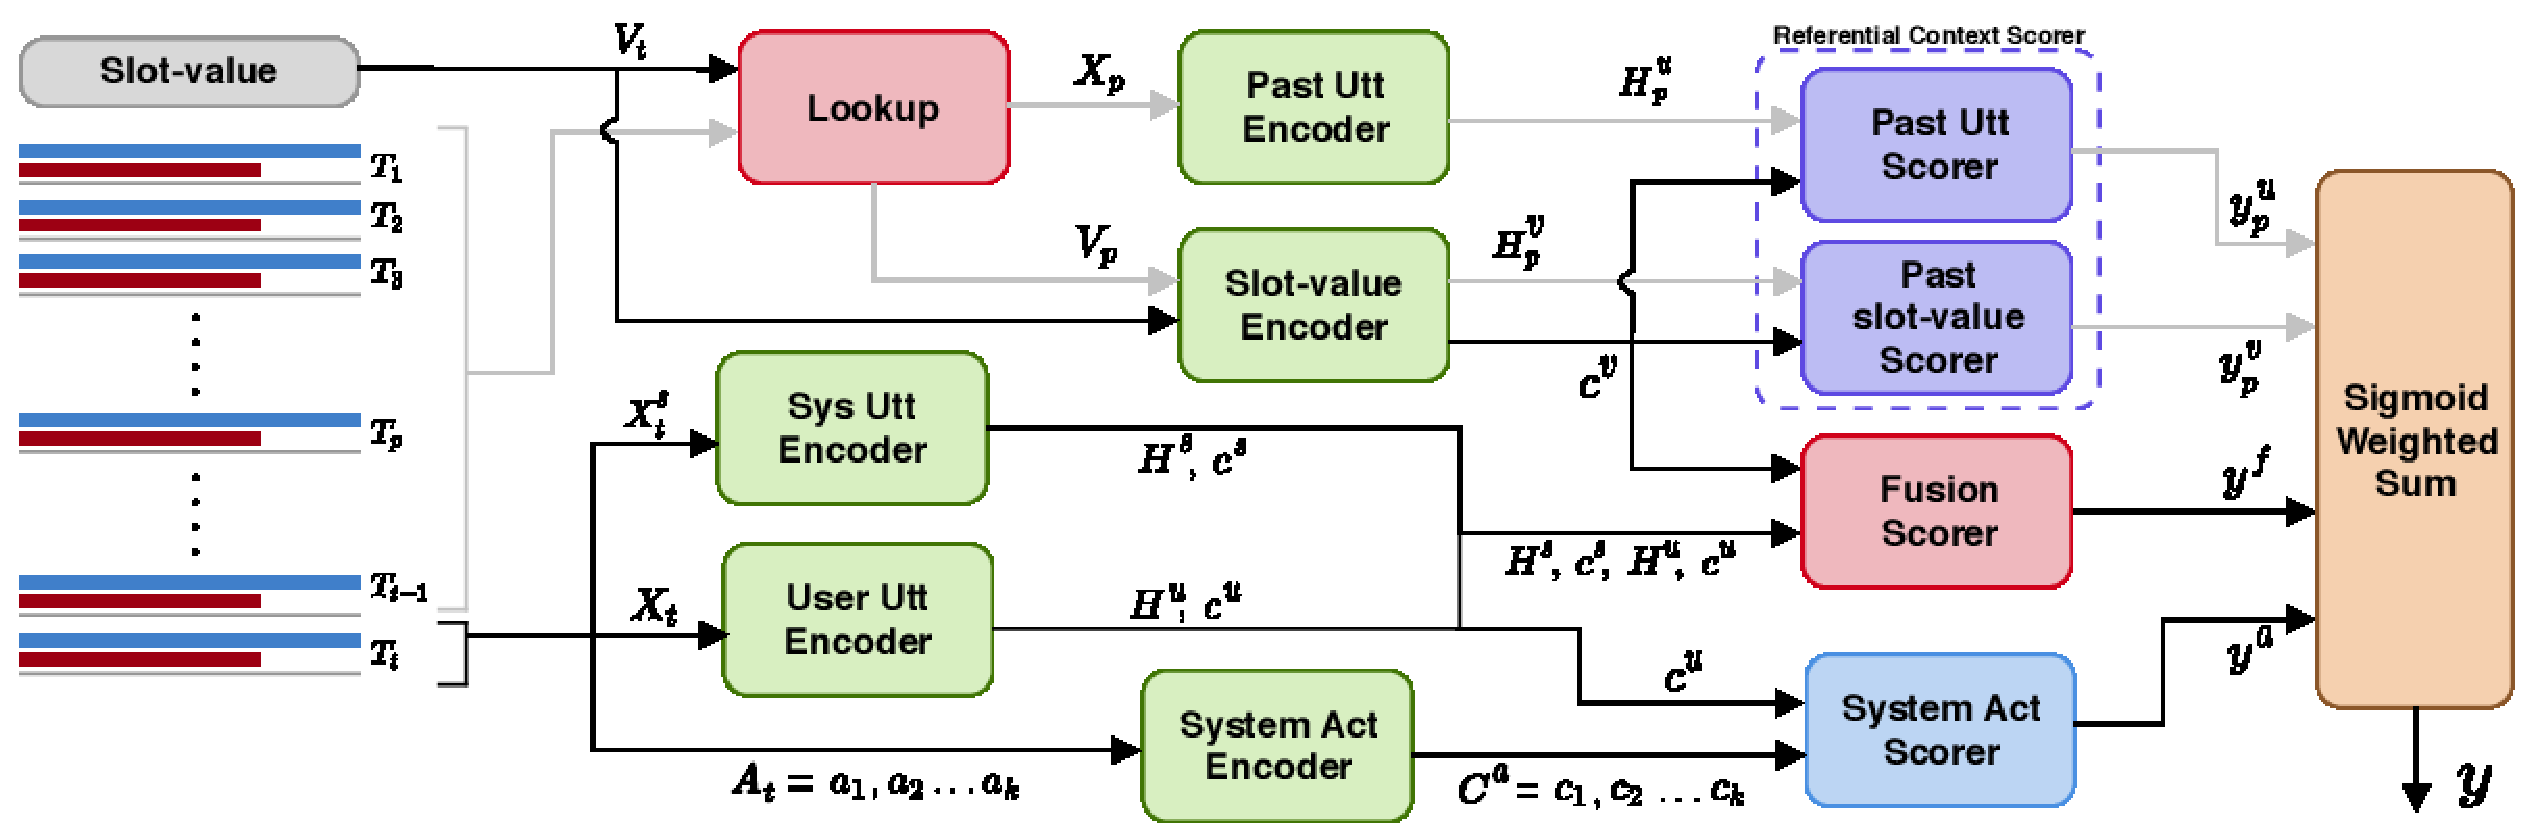
\includegraphics[width=15cm]{chapter4/kanren.eps}
      \caption{スロット抽出に関連する対話履歴を抽出するモデル図}
      \label{fig:kanren}
    \end{center}
\end{figure}

本研究は,対話履歴の使い方に関するものである.従来研究では,様々な方法で対話の流れを捉えようとしていた.例として,前のターンでのシステムの対話行為を入力に加える,前のターンの対話状態を入力に加える,過去数ターンの発話を入力に加えるなどがある.しかし,Sharma ら\cite{kanren} はこれらの手法では,ユーザが過去の発話に存在するスロット値を参照した時に対応できないこと,過去数ターンの発話を入力に加えるとノイズが増加することを指摘し,関連対話履歴を抽出する手法を提案した.この手法は,あるスロットの値を推定するときに,そのスロットの値を更新した発話を入力文に加えるものである.当時最先端のモデルであった GLAD モデル\cite{glad} に本手法を加えただけで性能を向上させることに成功した.
\par
本研究では,Sharma らの関連対話履歴を用いる手法に影響を受けて,対話行為を用いて重要な対話履歴を抽出する手法を提案する.